
\lstset{
language=csh,
basicstyle=\footnotesize\ttfamily,
numbers=left,
numberstyle=\tiny,
tabsize=2,
breaklines=true,
frame=b,
showspaces=false,
showtabs=false,
commentstyle=\color{green},
keywordstyle=\color{mauve},
morekeywords={lemma, method, function, predicate,ensures, requires, assert },
identifierstyle=\color{black},
backgroundcolor=\color{cloudwhite},
}

\chapter{Verificarea formală a problemei}

\section{Entry point-ul problemei}
    Un entry point este locația din cod în care se face transferul controlului, acolo se fac apelurile altor funcții ș.a.m.d.
    Implementarea algoritmului propriu-zis care rezolvă problema a fost primul și cel mai ușor pas.\par
    Am început prin crearea unei bucle care la fiecare pas alegea bancnota optimă, o adăuga în secvența de 
    bancnote considerată soluție și o scădea din sumă, fiind un algoritm tipic metodei greedy.
    \begin{lstlisting}
    var rest:= sum;
    solution:= [0, 0, 0, 0, 0, 0];
    while (0 < rest)
        decreases rest 
        {
        index:= maxBanknote(rest);
        var banknote:= power(2, index);
        solution:= addValueToIndex(solution,1,index);
        rest:= rest - banknote;
    }
    \end{lstlisting}

    Acest algoritm era suficient pentru a rezolva problema, dar nu era suficient pentru a demonstra că soluția produsă este optimă.\par
    Considerăm o soluție optimă soluția de cost minim, costul fiind numărul de bancnote.
    
\section{Demonstrarea optimalității}
    \subsection{Schema verificării}
    \vspace{1cm}
    \begin{center}
        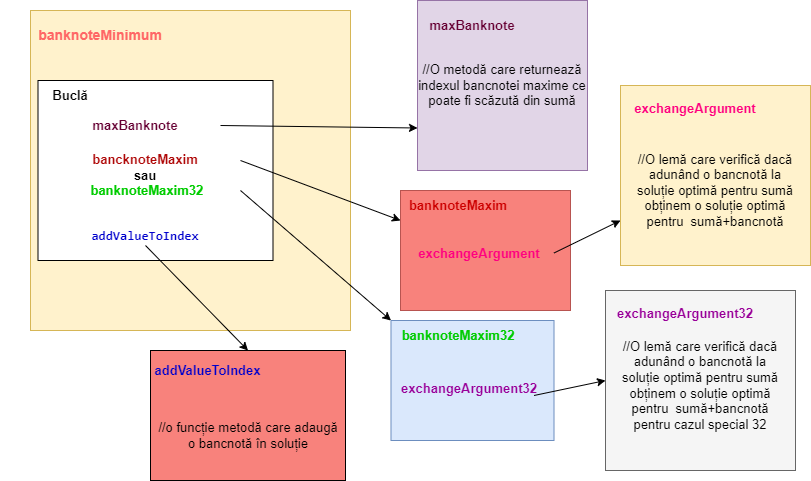
\includegraphics[width=1.0\textwidth]{verification_schema.png}\par
        \caption{Figura 1: o schemă explicativă a apelurilor de funcții și leme în cadrul verificării}
    \end{center}
   
    
\section{Etapele verificării}
Am implementat algoritmul greedy care rezolva problema bancnotelor cu bancnote puteri ale lui 2, 
apoi am adăugat treptat condițiile care garantează că soluția găsită este soluție optimă.
    \subsection{Metoda banknoteMinimum}
    Metoda banknoteMinimum returnează soluția optimă pentru o sumă dată ca input.\par
    Această metodă folosește o buclă, în care, la fiecare iterație, se adaugă o bancnotă în soluție.\par
    În primă fază calculează bancnota cea mai mare ce poate fi dată ca rest, cu ajutorul funcției maxBanknote și funcției 
    power.\par
    Ulterior, folosește lema banknoteMaxim sau banknoteMaxim32, în funcție de bancnota aleasă, pentru a demonstra 
    că soluția calculată până în prezent, adunată cu bancnota aleasă și cu o soluție optimă pentru $rest - bancnota$ 
    produce o soluție optimă pentru sumă .\par
    Proprietățile necesare unei soluții optime se păstreaza pe parcursul buclei cu ajutorul invariantelor.\par
     
    \begin{lstlisting}
    method banknoteMinimum(sum: int) returns(solution: seq <int> )
        requires sum >= 0
        ensures isValidSolution(solution)
        ensures isSolution(solution, sum)
        ensures isOptimalSolution(solution, sum) 
    {
        var rest:= sum;
        solution:= [0, 0, 0, 0, 0, 0];
        var index:= 0;
        assert isOptimalSolution(solution, sum - rest);
        while (0 < rest)
            invariant 0 <= rest <= sum
            invariant isValidSolution(solution)
            invariant addOptimRestEqualsOptimSum(rest, sum, solution)
            decreases rest 
        {
            index:= maxBanknote(rest);
            var banknote:= power(2, index);
            if (index != 5) 
            {
                banknoteMaxim(rest, sum, solution, index);
            } 
            else 
            {
                banknoteMaxim32(rest, sum, solution);
            }
            solution:= addValueToIndex(solution,1,index);
            rest:= rest - banknote;
        }
    }
    \end{lstlisting}

    \subsection{Metoda maxBanknote}
    Metoda maxBanknote este folosită pentru a returna un index cu proprietatea: \par
     $bancnota_{index} <= rest < bancnota_{index + 1}$  .\par
    \begin{lstlisting}
      method maxBanknote(sum: int) returns(index: int)
        requires sum > 0
        ensures 0 <= index <= 5
        ensures 0 <= power(2, index) <= sum
        ensures(index != 5 && power(2, index + 1) > sum) || index == 5 
      {
        index:= 5;
        if (power(2, index) > sum) 
        {
          assert power(2, index + 1) > sum;
          while (power(2, index) > sum && index > 0)
            invariant power(2, index + 1) > sum 
            {
              index:= index - 1;
              assert power(2, index + 1) > sum;
            }
        } 
          else 
        {
          assert index == 5;
        }
      }
    \end{lstlisting}


    \subsection{Lema banknoteMaxim}
    Lema banknoteMaxim este folosită pentru a demonstra faptul că dacă adăugam o bancnotă în soluția pe care o 
    construim, în continuare suma acestei soluții cu soluția optimă pentru $ rest - bancnota$ va produce soluția 
    optimă pentru suma întreagă.\par
    Pentru a demonstra acest lucru avem nevoie să știm că dacă în soluția curentă, optimă pentru $ rest - bancnota$  
    adaugăm bancnota aceasta devine optimă pentru $rest$.\par
    Acest lucru este demonstrat cu ajutorul lemei exchangeArgument.
    \begin{lstlisting}
    lemma banknoteMaxim(rest: int, sum: int, finalSolution: seq <int> , index: int)
        requires 0 <= index <= 4
        requires power(2, index) <= rest < power(2, index + 1)
        requires isValidSolution(finalSolution)
        requires addOptimRestEqualsOptimSum(rest, sum, finalSolution)
        ensures addOptimRestEqualsOptimSum(rest - power(2, index), sum, finalSolution[index:= finalSolution[index] + 1]) 
    {
        var banknote:= power(2, index);
        forall currentSolution | isValidSolution(currentSolution) && isOptimalSolution(currentSolution, rest - banknote)
            ensures isOptimalSolution(solutionsSum(solutionsSum(currentSolution, finalSolution), [0, 0, 0, 0, 0, 0][index:= 1]), sum) 
        {
            assert isSolution(currentSolution[index:= currentSolution[index] + 1], rest);
            exchangeArgument(rest, currentSolution, index);
        }
        assert forall currentSolution::isValidSolution(currentSolution) && isOptimalSolution(currentSolution, rest - banknote) ==> isOptimalSolution(solutionsSum(solutionsSum(currentSolution, finalSolution), [0, 0, 0, 0, 0, 0][index:= 1]), sum);
    }
    \end{lstlisting}

    \subsection{Lema exchangeArgument}
    Lema exchangeArgument presupune că nu este optimă soluția dacă adaugăm bancnota aleasă și ajunge la o contradicție.
    Știm că soluția e optimă pentru $rest - bancnota$, dar nu pentru rest, dacă adaugăm bancnota.\par
    Consideră că există o altă soluție optimă pentru rest.\par
    Verifică în presupusa soluție pentru rest că nu avem bancnota în soluție deja, altfel acea presupusă 
    $solutie - bancnota$ are cost mai mic decât soluția noastră care e optimă pentru $rest - bancnota$, contradicție.
    Apoi verificăm proprietatea descrisă la observație.\par
    Nu există două bancnote de aceeași valoare în soluție, mai mici de 32.\par
    În acest mod știm că soluția presupusă nu poate fi optimă, deoarece, dacă respectă proprietatea
    suma produsă de aceasta nu poate fi egală cu rest. \par
    Deoarece :\par
    $\bullet \sum_{k=0}^{index-1} 2^{k} = 2^{index}-1 $\par
    $\bullet rest > = 2^{index} $ \par
    Deci presupusa soluție pentru rest nu poate fi egală decât cu cel mult $rest-1$, astfel nu poate fi soluție optimă și se ajunge la o contradicție. 

    
    \begin{lstlisting}
lemma exchangeArgument(rest: int, currentSolution: seq <int> , index: int)
    requires 0 <= index <= 4
    requires power(2, index) <= rest < power(2, index + 1)
    requires isValidSolution(currentSolution)
    requires isOptimalSolution(currentSolution, rest - power(2, index))
    ensures isOptimalSolution(currentSolution[index:= currentSolution[index] + 1], rest) 
{
    var banknote:= power(2, index);
    var solution:= currentSolution[index:= currentSolution[index] + 1];
    assert isValidSolution(solution);
    assert isSolution(solution, rest);
    var i:= index;
    if (!isOptimalSolution(solution, rest)) 
    {
    var optimalSolution:| isValidSolution(optimalSolution) && isSolution(optimalSolution, rest) &&
        isOptimalSolution(optimalSolution, rest) && cost(optimalSolution) < cost(solution);
    if (optimalSolution[index] -1 >= 0) 
    {
        var betterSolution:= addValueToIndex(optimalSolution,-1,index);
        assert isSolution(betterSolution, rest - banknote);
        assert cost(betterSolution) == cost(optimalSolution) - 1;
        assert cost(optimalSolution) - 1 < cost(currentSolution);
        assert false;
    } 
    else 
    {
        while (0 < i)
        invariant 0 <= i <= index
        invariant forall x::index >= x >= i ==> optimalSolution[x] <= 1 
        {
        i:= i - 1;
        assert isOptimalSolution(optimalSolution, rest);
        if (optimalSolution[i] > 1) 
        {
            var optimalSolution' := optimalSolution[i:=optimalSolution[i]-2];
            optimalSolution' := optimalSolution' [i + 1:= optimalSolution'[i+1]+1];
            assert isSolution(optimalSolution', rest);
            assert cost(optimalSolution') == cost(optimalSolution) - 1;
            assert cost(optimalSolution') < cost(optimalSolution);
            assert false;
        }
        }
        assert solutionElementsSum(optimalSolution) <= banknote - 1;
        assert rest >= banknote; 
        assert solutionElementsSum(optimalSolution) <= rest - 1; 
        assert isOptimalSolution(optimalSolution, rest); 
        assert false;
        }
    }
}
    \end{lstlisting}
        
    
\subsection{Lema banknoteMaxim32}
Lema banknoteMaxim32 demonstrează proprietatea menționată anterior.\par
Știm că finalSolution este soluție optimă pentru $sum-rest$.\par
Dacă currentSolution la care adăugăm bancnota 32 este soluție optimă pentru $rest$, atunci suma soluției optime 
pentru $sum-rest$ adunată cu suma soluției optime pentru rest este soluție optimă pentru sumă.  \par
BanknoteMaxim32 se asigură că este soluție optimă pentru rest currentSolution folosind lema exchangeArgument32.

\begin{lstlisting}
lemma banknoteMaxim32(rest: int, sum: int, finalSolution: seq <int> )
    requires rest >= 32
    requires isValidSolution(finalSolution)
    requires addOptimRestEqualsOptimSum(rest, sum, finalSolution)
    ensures addOptimRestEqualsOptimSum(rest - 32, sum, solutionsSum(finalSolution, [0, 0, 0, 0, 0, 1])) 
{
    forall currentSolution | isValidSolution(currentSolution) && isSolution(currentSolution, rest - 32)
      ensures isSolution(solutionsSum(solutionsSum(finalSolution, currentSolution), [0, 0, 0, 0, 0, 1]), sum) 
    {
      assert isSolution(solutionsSum(currentSolution, [0, 0, 0, 0, 0, 1]), rest);
    }
  
    forall currentSolution | isValidSolution(currentSolution) && isOptimalSolution(currentSolution, rest - 32)
      ensures isOptimalSolution(solutionsSum(solutionsSum(finalSolution, currentSolution), [0, 0, 0, 0, 0, 1]), sum)
    {
      forall someSolution | isValidSolution(someSolution) && isSolution(someSolution, sum)
        ensures cost(someSolution) >= cost(solutionsSum(solutionsSum(finalSolution, currentSolution), [0, 0, 0, 0, 0, 1])) 
      {
        exchangeArgument32(rest, sum,  currentSolution);
      }
    }
}
\end{lstlisting}


\subsection{Lema exchangeArgument32}
Lema exchangeArgument32 presupune că nu este optimă soluția dacă adaugăm bancnota 32 și ajunge la o contradicție.\par
Știm că soluția e optimă pentru $rest - 32$, dar nu pentru rest, dacă adaugăm bancnota.\par
Consideră că există o altă soluție optimă pentru rest.\par
Deoarece nu avem o bancnotă mai mare de 32 cu care am putea înlocui 2 apariții ale acestei bancnote,
verificăm doar proprietatea descrisă la observație.\par
Nu există două bancnote de aceeași valoare în soluție, mai mici de 32.\par
În acest mod știm că soluția presupusă nu poate fi optimă, deoarece, dacă respectă proprietatea
suma produsă de aceasta nu poate fi egală cu rest. \par

\begin{lstlisting}    
lemma exchangeArgument32(rest: int, sum: int,  optimalSolution: seq <int> )
    requires 32 <= rest
    requires isValidSolution(optimalSolution)
    requires isOptimalSolution(optimalSolution, rest - 32)
    ensures isOptimalSolution(optimalSolution[5:= optimalSolution[5] + 1], rest) 
{
    var solution:= optimalSolution[5:= optimalSolution[5] + 1];
    var i:= 4;
    if (!isOptimalSolution(solution, rest)) 
    {
        if (optimalSolution[i] > 1) 
        {
            var solution:= optimalSolution[i:= optimalSolution[i] - 2];
            solution:= solution[i + 1:= solution[i + 1] + 1];
            assert isSolution(solution, rest - 32);
            assert cost(solution) == cost(optimalSolution) - 1;
            assert cost(optimalSolution) - 1 < cost(solution);
            assert false;
        } 
        else
        {
            while (0 < i)
                invariant 0 <= i <= 4
                invariant forall index::4 >= index >= i ==> optimalSolution[index] <= 1 
            {
                i:= i - 1;
                if (optimalSolution[i] > 1) 
                {
                    var solution:= optimalSolution[i:= optimalSolution[i] - 2];
                    solution:= solution[i + 1:= solution[i + 1] + 1];
                    assert isSolution(solution, rest - 32);
                    assert cost(solution) == cost(optimalSolution) - 1;
                    assert cost(optimalSolution) - 1 < cost(solution);
                    assert false;
                }
            }
            assert solutionElementsSum(optimalSolution) <= rest - 1;
            assert isOptimalSolution(solution, rest);
            assert false;
        }
    }
}

\end{lstlisting}

